\documentclass[a4paper,12pt,oneside]{scrreprt}
\usepackage[latin1]{inputenc}
\usepackage[english]{babel}
\usepackage{graphicx}
\usepackage{float}
\usepackage{geometry}
\geometry{verbose,a4paper,tmargin=25mm,bmargin=25mm,lmargin=15mm,rmargin=25mm}
\usepackage{paralist}

\usepackage{paracol}

\usepackage{todonotes}

\usepackage{listings}
\lstset{language=Java,
	tabsize=2,
	showspaces=false,
	showtabs=false,
	breaklines=true,
	showstringspaces=false,
	breakatwhitespace=true,
	commentstyle=\color{pgreen},
	keywordstyle=\color{pblue},
	stringstyle=\color{pred},
	basicstyle=\footnotesize\ttfamily,
	moredelim=[il][\textcolor{pgrey}]{$$},
	moredelim=[is][\textcolor{pgrey}]{\%\%}{\%\%}
}

\usepackage{tikz}
\usetikzlibrary{calc,patterns,angles,quotes}

\begin{document}


\begin{center}
	Submitted by Group 51
	
	\bigskip
	
	\begin{tabular}{ll}
	Group Members: \\
	CETIN, Ulfet (391819) \\
	GRUCZKA, FILIP () \\
	LIPINSKI, Bartosz () \\
	\end{tabular}

	\bigskip
	
	DIS1 WS 19/20 Assignment 1\\
	Predicting Human Performance using Fitts' Law
	
	%	(ordered on lastname basis)
\end{center}



\bigskip 

\begin{enumerate}

	\item  \mbox{}\\
	
		\begin{compactenum}
			\item \mbox{}\\
			
			\begin{compactitem}
				\item Distance from S to F , D$_{SF}$: 25 cm\\
				
				% TODO decide one of them
				\item Target Width for S to F , W$_{SF}$: 5 cm ( $\sqrt[2]{ 3^{2} + 4^{2} } = 5 $ )  \\
				
				
				
				
				\item Distance from F to C , D$_{FC}$: 32 cm\\
				
				\item Target Width for F to C , W$_{FC}$: 8 cm\\
				
					Shannon's formula for reference:	T$_{pos}$ = $ a + b * log_{2} (\frac{D}{W} + 1)$ \\
					given values: a = 0 ms, b = 100 ms/bit\\
					
					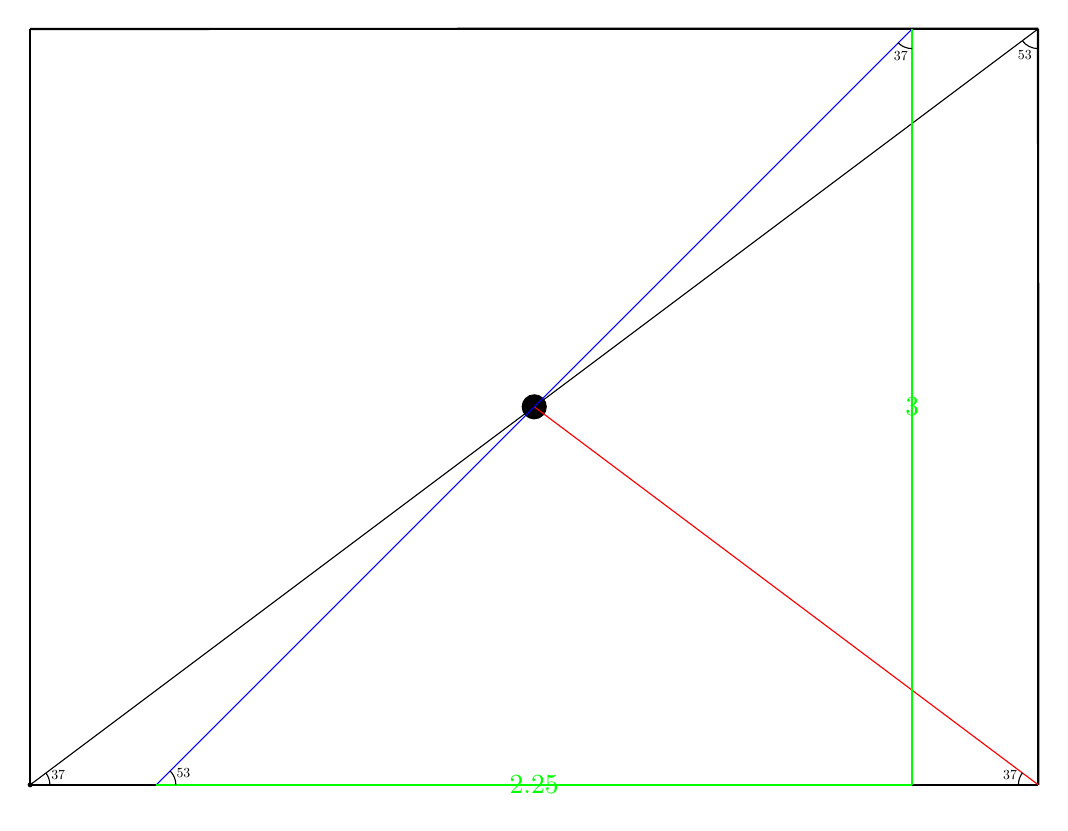
\begin{tikzpicture}[scale=3.2]
					\coordinate (lb) at (0,0);
					\fill[black] (lb) circle (0.01);
					
					\draw[thick] (lb) -- (4,0) coordinate (rb);
					\draw[thick] (rb) -- (4,3) coordinate (rt);
					\draw[thick] (rt) -- (0,3) coordinate (lt);
					\draw[thick] (lt) -- (lb);
					
					\draw (lb) -- (rt);
					
					\coordinate (center) at (2, 1.5);
					\fill[black] (center) circle (0.05);
					
					\draw[red] (rb) -- (center);
					
					\coordinate (a1) at (0.5,0);
					\coordinate (a2) at (3.5,3);
					\coordinate (a3) at (3.5,0);
					
					\draw[blue] (a1) -- (a2); 
					
					\draw[green, thick] (a2) -- (a3) node[midway] {3};
					
					\draw[green, thick] (a1) -- (a3) node[midway] {2.25};
					
					\pic [draw, "37"scale=0.5, angle eccentricity=1.5, scale=0.5] {angle = rb--lb--center};
					\pic [draw, "37"scale=0.5, angle eccentricity=1.5, scale=0.5] {angle = center--rb--lb};
					\pic [draw, "53"scale=0.5, angle eccentricity=1.5, scale=0.5] {angle = lb--rt--rb};
					
					\pic [draw, "53"scale=0.5, angle eccentricity=1.5, scale=0.5] {angle = rb--a1--center};
					\pic [draw, "37"scale=0.5, angle eccentricity=1.5, scale=0.5] {angle = a1--a2--a3};
					\end{tikzpicture}
					
					Length of the blue line (that is perpendicular to red line) is 3.75 cm.\\
					\clearpage
					
				
				\item Movement Time for S to F , MT$_{SF}$:\\
				 MT$_{SF}$ = $ 0 ms + 100 \frac{ms}{bit} * log_{2} (\frac{25}{5} + 1)$ = 258.49625007211563 ms
				\\
				
				\item Movement Time for F to C , MT$_{FC}$:\\
				MT$_{FC}$ = $ 0 ms + 100 \frac{ms}{bit} * log_{2} (\frac{32}{8} + 1)$ = 232.19280948873623 ms
				\\
				
				\item Movement Time for S to C , MT$_{SC}$: \\
				MT$_{SC}$ = 258.49625007211563 + 232.19280948873623 = 490.6890595608519 ms
				\\
			\end{compactitem}
			
			
			
			\item Using fingers (b) instead of mouse (a) causes the movement time to: \textbf{DECREASES}.
			r1 = 100 + 50*log(25.0/5 + 1, 2)\\
			r2 = 100 + 50*log(32.0/8 + 1, 2)\\
			r1 + r2 $\rightarrow$ 445.3445297804259 ms
			
		\end{compactenum}
	
		\bigskip
	
	\item Sketch of your redesign:
	
		\begin{figure}[h]
			\centering
			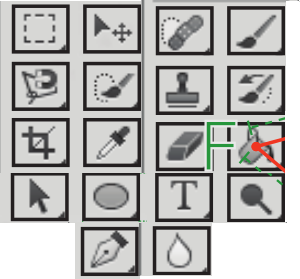
\includegraphics[clip, trim=0cm 0cm 0cm 0cm, scale=0.9]{./images/q2v3.png}
		\end{figure}
	
		\bigskip
		
		How your redesign minimizes the selection time:\\
		
		The buttons are ordered in the toolbox that is closer to a square form, compared to the original (that is in rectangular form). The square form reduces the time required to access the buttons (especially edge cases) drastically. In previous rectangular form that is longer in height, accessing to the buttons that are on the upper side of the toolbox was higher, or on the bottom side, based on where the cursor is. Still, wherever the cursor is, it does not help being longer in the height (neither in the width, for that matter). All in all, square-like form of ours, compared to original one, cuts down the average time required to access buttons drastically.
		
		
	\clearpage
		
	\item \mbox{}
		\bigskip
		\begin{compactitem}
			\item Argument \#1:
			
			\bigskip
			
			\item Argument \#2:
		\end{compactitem}
	

	
\end{enumerate}


\end{document}}
